\documentclass{beamer}
\usepackage[utf8]{inputenc}
\usetheme{Madrid}
\usecolortheme{default}
\usepackage{hyperref}
\usepackage{tikz}
%------------------------------------------------------------
%This block of code defines the information to appear in the
%Title page
\title[TIPE]{Un Algorithme De Covoiturage ?}
\subtitle{La ville}
\author[A. Belfkira]{Amin Belfkira}
\institute{Candidat 12135}
\date{}






             %End of title page configuration block
             %------------------------------------------------------------



             %------------------------------------------------------------
             %The next block of commands puts the table of contents at the
             %beginning of each section and highlights the current section:


             %------------------------------------------------------------


\begin{document}

%The next statement creates the title page.
\frame{\titlepage}


%---------------------------------------------------------
%This block of code is for the table of contents after
%the title page
\begin{frame}
  \frametitle
  {Sommaire}
  \tableofcontents
\end{frame}
%---------------------------------------------------------


\section{Contexte}
\begin{frame}{Contexte}

  Les déplacements posent de plus en plus de contraintes aux usagers : durée, coût, pas pratique...
  \newline
  \textbf{Avantages du covoiturage :}
  \begin{itemize}
    \item Flexible
    \item Economique : peu onéreux pour le passager, rentable pour le conducteur
    \item Social: création de liens avec des voisins, collègues...
    \item Environnemental : limite le nombre de voitures et réduit les émissions
  \end{itemize}

  \textbf{Objectif:} Créer une solution de covoiturage avantageuse pour le conducteur et le passager


\end{frame}

%---------------------------------------------------------

\begin{frame}{Problème}

  Mettre en relation deux utilisateurs :déterminer le lieu de rencontre $x_{in}$ et de séparation $x_{off}$ un piéton et un conducteur possédant un point de départ et d'arrivée $d_p$ $a_p$ et $d_c$, $a_c$
  \begin{center}
    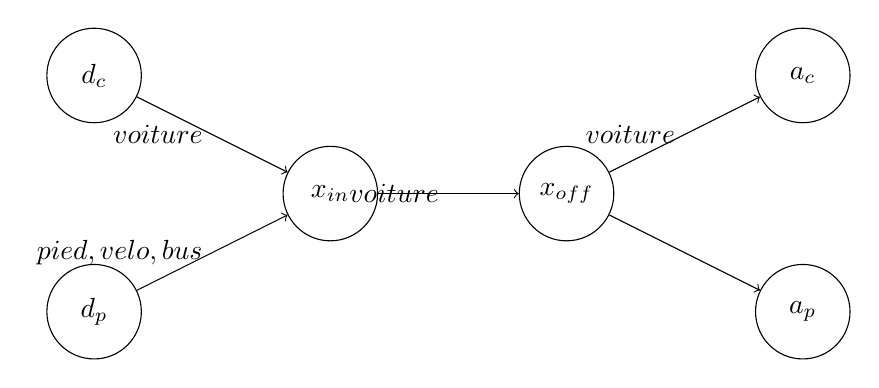
\begin{tikzpicture}
      \node[shape=circle,draw=black,minimum size=1.2cm] (0) at (0,1.5) {$d_c$};
      \node[shape=circle,draw=black,minimum size=1.2cm] (1) at (3,0) {$x_{in}$} ;
      \node[shape=circle,draw=black,minimum size=1.2cm] (2) at (0,-1.5) {$d_p$} ;
      \node[shape=circle,draw=black,minimum size=1.2cm] (3) at (9,1.5) { $a_c$} ;
      \node[shape=circle,draw=black,minimum size=1.2cm] (4) at (9,-1.5) { $a_p$} ;
      \node[shape=circle,draw=black,minimum size=1.2cm] (5) at (6,0) {$x_{off}$} ;
      \path [->](0) edge node[left] {$voiture$} (1) ;
      \path [->](2) edge node[left] {${pied, velo, bus}$} (1) ;
      \path [->](5) edge node[left] {$voiture$} (3) ;
      \path [->](5) edge node[left] {} (4) ;
      \path [->](1) edge node[left] {$voiture$} (5) ;

    \end{tikzpicture}
  \end{center}



\end{frame}
%---------------------------------------------------------
\section{Modélisation}

\begin{frame}
  \frametitle{Modélisation}


  \begin{itemize}
    \item Graphe non orienté pondéré et étiqueté, dont le poids est la durée du trajet entre deux sommets et l'étiquette le moyen de locomotion
    \item Données utilisées :
          \begin{itemize}
            \item Routes : OpenStreetMap de la région Rhônes-Alpes
            \item Transports en commun : Open Data du Grand Lyon
          \end{itemize}
    \item Implémentation : Python et C
    \item Modèle dépendant du temps ?
  \end{itemize}
\end{frame}
%---------------------------------------------------------

\section{Résolution}

\begin{frame}
  \frametitle{Résolution du problème}

  Méthodes et procédés envisagées pour déterminer la durée de trajet minimale entre chaque sommet :

  \begin{itemize}
    \item Automate Fini Non Déterministe NFA pour déterminer les contraintes
    \item Algorithme de Dijkstra appliqué au sous-graphe déduit des contraintes
    \item Files de priorité implémentées par tas
    \item Algorithme A*
  \end{itemize}
\end{frame}

\begin{frame}
  \frametitle{Déterminer le point de rendez-vous}

  Les distances minimales entre deux sommets désormais connues, il reste à déterminer un point de rendez-vous entre le conducteur et le passager en minimisant le temps de trajet de chacun.
  \newline
  Procédé envisagé :
  \begin{itemize}
    \item Déterminer tous les points de rencontre possibles et leur associer un coût : la somme des poids des arêtes parcourues
    \item Plusieurs origines possibles : Algorithme de Dijkstra non adapté
    \item Utilisation de l'algorithme de Martins
    \item Ajout de contraintes spécifiques de l'utilisateur
  \end{itemize}
\end{frame}

\begin{frame}
  \frametitle{Pistes}

  \section{Pistes à exploiter}
  Elements à réaliser et pistes à explorer :
  \begin{itemize}
    \item Implémentation
    \item Evolution du modèle :
          \begin{itemize}
            \item Passer de 2 à N participants ?
            \item Modèle dépendant du temps ?
          \end{itemize}
    \item Complexité
    \item Tests
    \item Ajout d'une interface graphique ?
  \end{itemize}
\end{frame}

\begin{frame}
  \frametitle{Bibliographie}
  \section{Bibliographie}
  \begin{itemize}
    \item \textit{A Fair Carpool Algorithm}, R. Fagin \& J. Hagins
    \item \textit{Algorithms For The Carpooling Problem}, A. Bit-Monnot

    \item \textit{Minimizing the average arriving distance in carpooling},
          T. Zhao \& Y. Yang \& E. Wang

    \item \url{https://data.grandlyon.com/jeux-de-donnees/reseau-transport-commun-lyonnais/info}
    \item \url{https://www.openstreetmap.fr/donnees/}
  \end{itemize}
\end{frame}


%---------------------------------------------------------
%Highlighting text

%---------------------------------------------------------


%---------------------------------------------------------
%Two columns
%---------------------------------------------------------


\end{document}
